\section{Design Decisions and Technology Stacks} \label{TS} 
This chapter deals with fundamental concepts and technology stacks used for developing our decentralized supply chain management system. This system is described in chapter \ref{usecase}. The backbone of our system is a Smart Contract running on Ethereum. In addition to tracking goods, our system is also used for managing costs and paying suppliers for their services. This system employs Raiden Network \ref{IPFS} based payment channels to securely handle financial transactions. InterPlanetary File System is used for storing large documents and complete logs related to individual supply chain processes. 
 
%This chapter ends with a short description of the Quantum computing threat to blockchains and the need for decentralized applications to be resilient against Quantum attackers \ref{Qsig}.
\vspace{0.5cm}
\subsection{Ethereum}\label{eth}
Ethereum is a decentralized blockchain based computing platform that provides Smart Contract functionality. It aims to be a platform for building decentralized applications (Dapps). Ethereum has a decentralized Turing Complete virtual machine which serves as an abstract foundation layer for building Dapps and running Smart Contracts. The Ethereum Virtual Machine (EVM) is programmed using a programming language called Solidity.
\subsection*{Motivation}
Ethereum was selected as it is the largest and most secure platform for Smart Contracts and decentralized applications available as of the writing of this thesis. Its open source nature and other design philosophies like Simplicity, Universality, Modularity, Agility and Non-Censorship were also important considerations in favor of its selection \cite{eth:001}. Ethereum is special because each block in its blockchain represents a state of its virtual machine \cite{eth:001}. The design philosophy of Ethereum follows a set of principles outlined below:

\textbf{Simplicity:} The Ethereum Protocol is designed to be as simple as possible to fully realize the unprecedented democratization potential of blockchains \cite{eth:001}. 

\textbf{Universality:} Ethereum provides a Turning Complete scripting language.  Programmers can use this language to develop any Smart Contract, which can be mathematically defined.  Ethereum does not have “features”, instead its design philosophy follows the principal: If it can be correctly defined mathematically, then it can be built on Ethereum \cite{eth:001}. 

\textbf{Modularity:} The Ethereum protocol is designed to be as modular and separable as possible. This insures that small changes to the protocol do not affect applications that are already running on Ethereum. That is why Ethereum mining algorithm and consensus mechanisms are designed as separate modules \cite{eth:001}. This is one of the reasons that Ethereum is perfectly poised to adequately meet the scaling challenges facing public blockchains. Designers are already working on multiple scaling solutions including Plasma, Sharding, and Raiden.

\textbf{Agility:} The Ethereum protocol is designed to be modifiable in order to meet the security and scalability challenges of the future. Though designers and developers are extremely judicious about making changes to high-level constructs. However, if during testing and development process developers discover that changes to protocol architecture or EVM may lead to substantial improvements, they are quick to exploit them \cite{eth:001}. 

\textbf{Non-Censorship:} The protocol is designed to be application agnostic. It does not restrict specific categories of usage. All regulatory mechanisms are designed to prevent harm to the network as opposed to restrict any undesirable application \cite{eth:001}.
\vspace{0.5cm}  
\subsection*{Architecture Elements of Ethereum}
\subsubsection{Ethereum virtual machine}
The Ethereum Virtual Machine presents an abstract architecture to run Smart Contracts on different mining hardware setups all over the world. EVM serves as the run time environment for Smart Contracts on Ethereum. It prevents programs from accessing each other’s state and ensures that communication can be established without any interference. It is completely isolated from the rest of the main network and as such can be used as a perfect testing environment \cite{misc:023}.
\vspace{0.5cm}  
\subsubsection{Merkle Trees in Ethereum}
Merkle Trees are an important part of any blockchains as described in \ref{MerkleTrees}.  The purpose of Merkle Trees is to efficiently verify the data in a block without creating giant block headers, which would have adverse effects on blockchain scalability and decentralization. In Bitcoin each block header contains one tree structure to represent transactions \cite{misc:025}. Ethereum, on the other hand uses Merkle trees (see fig \ref{fig:EthTree}) to represent three kinds of objects \cite{misc:025}:

\begin{itemize}
\item Transactions 
\item Receipts
\item State
\end{itemize}

\begin{figure}[h]
	\centering
    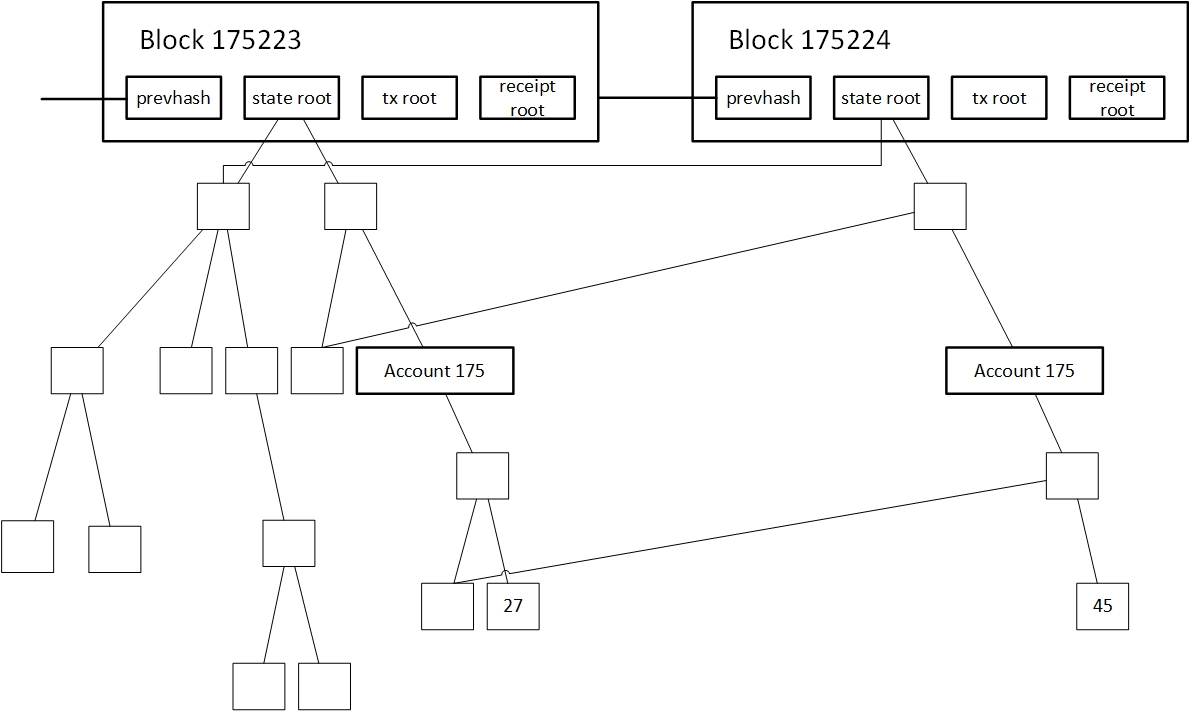
\includegraphics[width=130mm,scale=1]{figs/ethtree}
	\caption{Merkle Trees in Ethereum \cite{misc:025}}
	\label{fig:EthTree}
\end{figure}

Each tree in Ethereum handles a specific type of query. A Transaction tree is used to verify if a particular transaction has been included in a block or not.  A Receipt tree handles events. It can be used to get all instances of a particular event X emitted by a particular address over a period of time for e.g. last 30 days. A State tree is used to confirm validity and existence of an account and its balance. These trees function in a highly efficient manner, in most cases it is just a matter of fetching the correct Merkle branch and replying back to the client.  Together these three trees allow for the creation of a highly advanced yet light protocol which can be executed by light clients to create a highly decentralized computing network \cite{misc:025}. 
 
Ethereum uses a special form of Merkle tree called Patricia trees \cite{ethwiki:007}. These are more complex data structures compared to the binary trees used in Bitcoin. Binary Merkle trees are a good data structure for creating transaction trees as the tree is created once and then frozen solid. The state in Ethereum however needs to be frequently updated. This requires a data structure where the root can be quickly calculated after each insert, edit, update or delete operation without reconstructing the entire tree. The state in Ethereum is basically a key – value mapping where the key is the account address and value is a combination of account balance, nonce, code and storage for each address. Storage itself is a tree as well \cite{misc:025}.The Patricia tree is the most suitable data structure for the Ethereum protocol. Detailed specifications for these trees is presented in \cite{ethwiki:007}. \textit{“The simplest explanation for how it works is that the key under which a value is stored is encoded into the path that you have to take down the tree. Each node has 16 children, so the path is determined by hex encoding: for example, the key dog hex encoded is 6 4 6 15 6 7, so you would start with the root, go down the 6th child, then the fourth, and so forth until you reach the end”} \cite{misc:025}. Patricia trees have highly desirable secondary properties as well: 
 
\begin{itemize}
\item They have bounded depth even in the presence of an attacker, who is deliberately trying to craft transactions to make the tree as deep as possible. This prevents denial of service attacks, which would be possible if each individual update became extremely slow due to large size of the tree \cite{misc:025}.  
\item The root of the tree only depends upon the data in the tree and not the orders in which updates are made \cite{misc:025}.
\end{itemize}
\clearpage

\subsubsection{Ethereum State Transition Function}
Technically any blockchain based ledger can be thought of as state transition function. Ethereum State Transition Function APPLY(S,TX) $\rightarrow$ S’ represented by the figure \ref{fig:EthSTF} works as follows \cite{eth:001}

\begin{enumerate}
\item Check if the signatures are valid and the nonce matches with senders nonce \cite{eth:001}.
\item Calculate Gas to pay for the transaction, subtract the gas price from senders account and increment senders nonce i.e. transaction count for senders account \cite{eth:001}.
\item Initialize gas and pay for transaction by taking off certain quantity of gas per byte for each byte in the transaction \cite{eth:001}.
\item Execute the transaction, if transaction is transfer function then move coins from senders account to receiver account. If the transaction is to a contract address, execute the contract code to completion or until execution runs out of gas \cite{eth:001}.
\item If the transaction failed due to not having enough coins or code execution running out of gas revert all state changes \cite{eth:001}.
\item Revert any remaining gas to the senders account \cite{eth:001}.
\end{enumerate}

\begin{figure}[h]
	\centering
    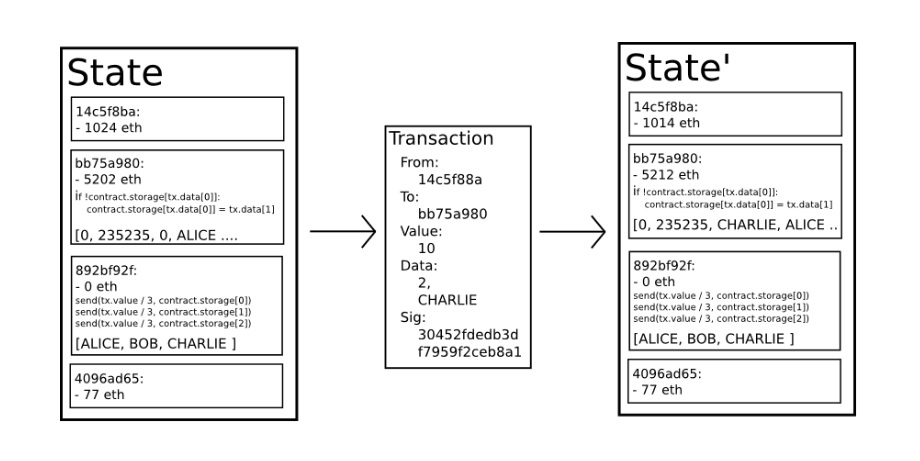
\includegraphics[width=180mm,scale=1]{figs/ethstf}
	\caption{Ethereum State Transition Function \cite{eth:001}}
	\label{fig:EthSTF}
\end{figure}
\clearpage
%https://github.com/ethereum/wiki/wiki/White-Paper#ethereum
\subsubsection{Block limits and Gas} \label{trxprice} 
Block Limits and Gas are regulatory mechanisms to prevent network abuse. These measures are designed to restrict and discourage attack vectors, without censoring nodes and users. 
 
\textbf{Gas}
Transactions on Ethereum network cost Gas. Users pay for each transaction in Eth, which is the native currency of the Ethereum protocol. Each operation on Ethereum costs different amounts of gas to execute. The gas price is directly related to the computational complexity of the operation to be performed. Every transaction includes two parameters ‘Gas Limit’ and ‘Gas Price’.  The gas limit is the maximum gas a user is willing to pay for executing a transaction, and gas price is the price of basic unit of gas called ‘wei’ in Eth. The total cost of a transaction in Eth is given by the following equation: \cite{eth:001}
\[ Total Transaction Cost = GasUsed * GasPrice \]

\textbf{Block Limits}
The block limit determines how many transactions or operations can fit into any one block. It puts an upper limit on the maximum amount of gas per block. If the block limit is 100 gwei and average transaction costs 20 gwei than a total 5 transactions can fit into a single block. Block limits are created to mitigate infinite loop attacks and malicious denial of service (DoS) attacks. A malicious DoS happens when an attacker creates multiple transactions that are cheap to add to the network but have operations that are computationally difficult to execute for clients. This results in network slowing down due to many pending transactions and consistently full blocks \cite{misc:026}. Block limits are configurable, Ethereum protocol provides a built in mechanism for changing block limits where by miners can vote on the new block limits. This allows to increase the capacity without requiring a hard fork \cite{eth:001}.
 
%\clearpage
\vspace{0.5cm}
\subsection{Smart Contracts}
Smart Contracts are computer programs that autonomously executes a set of functions or events based on predefined conditions. They allow automatic exchange of goods and services be it money, property, shares or anything of value in a conflict-free way avoiding middlemen. Smart Contracts can be used in all sorts of scenarios like financial services, crowd funding (ICOs), credit enforcements etc \cite{paper:009}. A generic Smart Contract can be represented by a transition diagram illustrated in figure \ref{fig:smartcontract}. This figure can be explained with the help of the example given below.
 
\textbf{Example:}
This example details a blockchain based property rental service. The user rents an apartment through a service which uses Ethereum blockchain to facilitate payments and   key transfers. Properties are listed on a Smart Contract with rental conditions like duration of stay and price per night already stipulated in the terms of the contract (see fig \ref{fig:smartcontract}). The tenant can agree to the terms by paying for the duration of his stay in cryptocurrencies. The payment will trigger associated events in the smart contract (see fig \ref{fig:smartcontract}).  Funds are blocked by the contract until the tenant receives the key. The key can be transferred digitally or physically. If the key doesn’t arrive, the contract releases the funds back to the tenant. If the key arrives, the contract transfers the funds to the owner of the property. The contract is automatically executed and cannot be interfered by either party. The contractual terms are implicitly agreed to by both parties and are witnessed by hundreds of people / miners \cite{misc:024}.   

\begin{figure}[h]
	\centering
    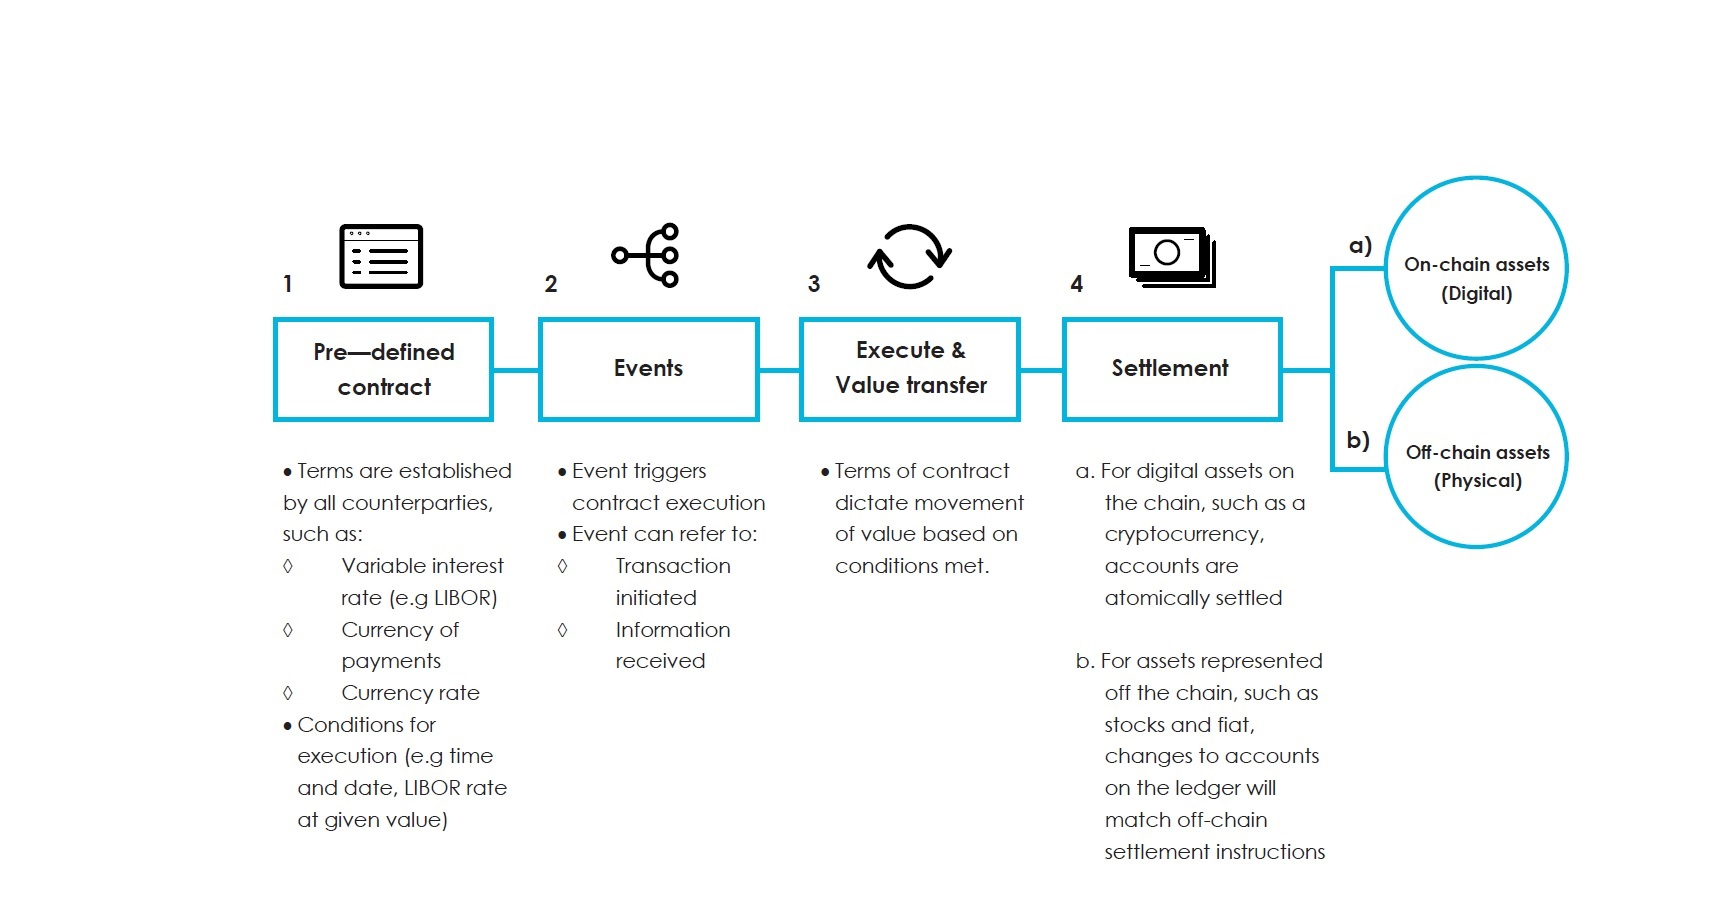
\includegraphics[width=180mm,scale=0.5]{figs/smartcontract}
	\caption{Smart Contract \cite{paper:009}} 
	\label{fig:smartcontract}
\end{figure}
%\clearpage
\vspace{0.5cm} 
\subsubsection{Interacting with Ethereum Smart Contracts}
Smart Contracts on Ethereum are written in Solidity which is a statically typed, contract oriented high-level programming language, developed to target the Ethereum Virtual Machine. Decentralized applications are composed of multiple modules, including modules for interacting with Smart Contracts and other traditional programming functions like GUIs etc. In order to facilitate Dapp development, Ethereum developers created an Application Binary Interface (ABI) to serve as a bridge between Smart Contracts and the rest of the application code. This ABI exposes Smart Contract functions to other application modules, that are developed for traditional environments using common programming languages like JavaScript (Web3), Python (Pyethereum.py), and Go.  To facilitate decentralized application development Ethereum provides a number of helper libraries including Web3 for JavaScript and Pyethereum for Python. These helper libraries use the Ethereum ABI to interact with Smart Contracts running on the Ethereum Virtual Machine or EVM. ABI is generated by compiling Solidity code. %A sample solidity contract is given below in Listing \ref{lst:label}. 


%------------------------------------------------------------------------------
%describe what smart contracts are and what they can do
%write about eVM, solidity, and how to communicate with smart contracts from %dapps i.e. web3 py3 etc
%create a graphical figure showing interaction between smart contract and web3 dapp


%\subsubsection{Future Roadmap}
%\subsubsection{Casper}
%https://github.com/ethereum/wiki/wiki/Proof-of-Stake-FAQs
%\subsubsection{Sharding}
%\subsubsection{Plasma}
%\subsubsection{State channels - Raiden Network}
%subsubsection{Virtual Channels - Perun}
%use the already made text from the other file for Raiden and Perun
%text goes here....



\subsection{Raiden Network} \label{raiden} 
Raiden network aims to solve the scaling problem described in \ref{scaling} for the Ethereum blockchain. Raiden was chosen as it was the most stable off chain payment solution available at the time of writing. It uses Payment Channels and payment Routing to perform ERC20 token transfers in an off chain manner.  Payment Routing is a technique to transfer token between two participants who do not have direct connection or channel with each other. This technique advocates using a network of interconnected channels and multi hop transfers to find a path between the participants. An abstract representation of a bidirectional Raiden payment channel is shown in figure \ref{fig:RPC}. 

\begin{figure}[h]
	\centering
    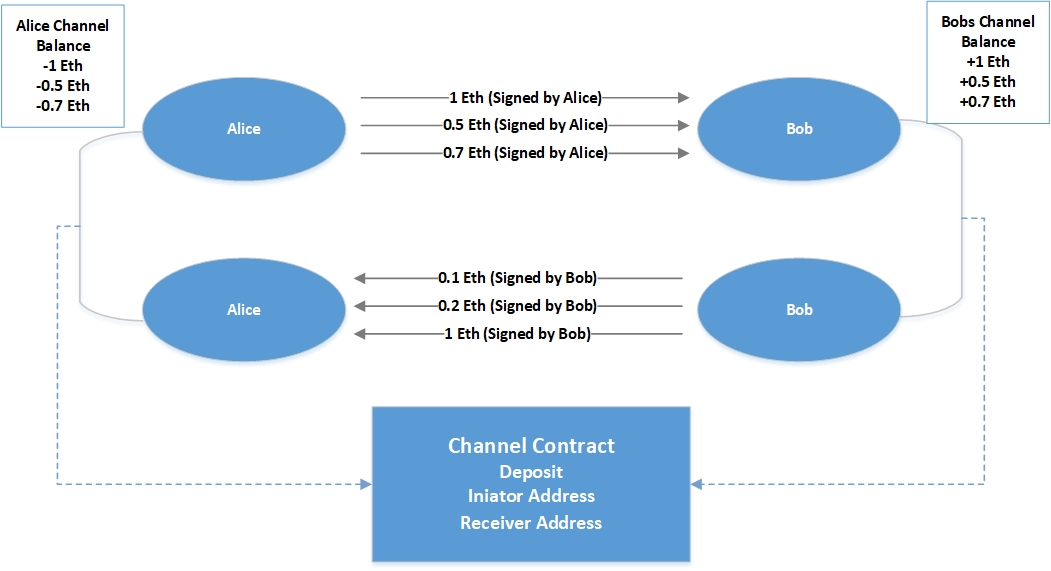
\includegraphics[width=140mm,scale=1]{figs/RPC}
	\caption{Bidirectional Payment Channel}
	\label{fig:RPC}
\end{figure}
%\clearpage

This figure shows a direct channel between Alice and Bob. The channel can be opened by any participant by deploying the channel contract (see \ref{NCSC}) on the Ethereum blockchain. The channel contract contains a deposit and two Ethereum addresses i.e. receiver address and iniator address. Once the channel is established, participants can make multiple transfers to each other by signing transactions within the channel. Each signed transaction updates the balance of the channel participants as shown in figure \ref{fig:RPC}. The channel can be closed at any point by either participant by putting the last signed transaction of the counter party on the blockchain. The channel contract then executes on the blockchain: it closes the channel and updates the final balance of the participants \cite{rad:001}. This was an example of direct transfer between two participants, however, in order for the network to scale it needs to provide a method for transferring coins between participants, who do not have a direct channel with each other. Raiden accomplishes this by using so called Mediated transfers shown in figure \ref{fig:PaymentRouting}. Mediated transfers can be used in our system to pay shippers by initiating a mediated transfer using suppliers. Mediated transfers are completed using Payement Routing (see \ref{NP}). Payment Routing relies on Hash Locked Transfers described in \ref{LN} to transfer coins between participants, who do not have a direct connection with each other. In the example shown in figure \ref{fig:PaymentRouting} Alice can transfer coins to Trudy even though she does not have a direct channel with her. This is accomplished by leveraging a path through the Raiden Network relying on intermediate connections that facilitate multi hop transfers \cite{rad:001}.  Sections \ref{NCSC}, \ref{CLC}, \ref{RaidenTrans}, \ref{NP}, and \ref{R-API} briefly explain important modules and building blocks of the Raiden Network.

\begin{figure}[h]
	\centering
    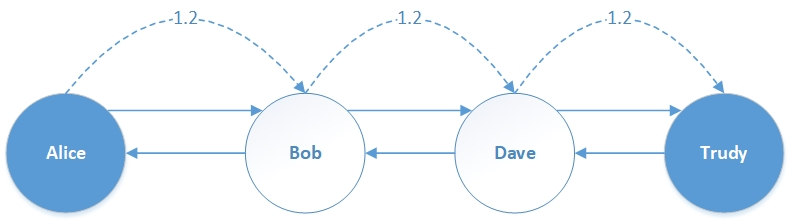
\includegraphics[width=120mm,scale=1]{figs/PaymentRouting}
	\caption{Payment Routing}
	\label{fig:PaymentRouting}
\end{figure}
\vspace{0.5cm}
\subsubsection{Netting Channel Smart contract} \label{NCSC}	
Netting Channel Smart Contract is Raiden’s implementation of a Payment Channel Contract. This contract gets deployed on the Ethereum blockchain when a channel is created. It carries shared rules implicitly agreed upon by the participants of an off-chain channel. It allows for the following: \cite{rad:001}
\begin{itemize}

\item Arbitrary number of token/asset transfers between channel participants \cite{rad:001}.
\item Conditional value transfers that have an expiration and predefined rule to withdraw \cite{rad:001}.
\item Rules to determine order of transfers \cite{rad:001}.

\end{itemize}
Each Netting Channel is associated with one bi-directional payment channel. Each channel deals with an ERC20 token and has its own settlement period measured in terms of blocks. ERC20 is a token standard for defining custom tokens or coins on top of Ethereum blockchain. Participants can deposit the associated type of ERC20 token any number of times at any time after the channel is opened. The token transfers are represented by lock structures that contain token amount, expiration and hash lock. The set of pending transfers are encoded into a Markel tree and represented in each transfer by its root. The total channel capacity is equal to total amount of tokens deposited by both participants. Any participant can increase the capacity at any time by depositing more tokens into the channel. The capacity is divided into available and locked balance to each participant/direction \cite{rad:001}.
%\vspace{0.5cm}
\clearpage
\subsubsection{Channel Life Cycle} \label{CLC}	
A Payment Channel in Raiden can be in one of the following stages of its lifecycle.
\begin{itemize}

\item Deployement
\item Funding / Usage
\item Close
\item Settle
\end{itemize}
\textbf{Deployement:} A channel is deployed by calling the textit{/channel} endpoint of Raiden Rest API with the correct ERC20 token address and the partner address with whom the channel needs to be created \cite{rad:001}.

\textbf{Funding:} A channel can be funded by either party by transferring and locking tokens in the channel. Once tokens have been transferred each participant can perform an arbitrary number of transfers back and forth provided they have the necessary funds to perform the transfer. A channel user can transfer token to another user by calling the textit{/transfer} end point as described in \ref{R-API} \cite{rad:001}.

\textbf{Close:} Once either party wants to withdraw tokens or a dispute arises the channel must be closed. This is done by calling the close function. After the close function is called the settlement window opens. The settlement window is the number of blocks participants have to wait before outstanding balance is settled on the blockchain. Within the settlement window both parties must update the counterparty state and withdraw the unlocked locks \cite{rad:001}.

\textbf{Settle:} Any participant can close the channel at any point. From that point no more transfers can be made. Once the channel enters the settlement window the partner state can be updated using the textit{updateTransfer()} function. After partner state is updated any outstanding locks may be withdrawn. A withdraw checks the locks and updates the participants current transferred amount. Once the withdraw is called or settlement timeout expires, the final tokens locked in the channel are distributed to the partners according to final balance of each party in the channel\cite{rad:001}. 
%\vspace{0.5cm}
\clearpage
\subsubsection{Token Transfer Types} \label{RaidenTrans}
Raiden Network supports three types of token transfer within its payment channels. These are Directed Transfer, Mediated Transfer, and Refund Transfer.

\textbf{Direct Transfer:} A direct transfer does not rely on locks. It is automatically completed as soon as the sending party sends the transfer packet containing the signed authorization for the transfer of coins. Trust is assumed between payer and payee. Sender assumes that transfer is complete after sending the transfer packet. The counterparty sends acknowledgment on receiving the message but due to the nature of the underlying network infrastructure either the sending message or the acknowledgement can get lost \cite{rad:001}.

\textbf{Mediated Transfer:} A mediated transfer is basically a hash locked transfer. The lock has an amount that needs to be transferred, a hash lock to verify the secret that unlock the amount and a validity period \cite{rad:001}. Mediated transfers have a sender address, a receiver address and a parameter to determine the number of hops between the two. The number of hops can be zero for direct transfers \cite{rad:001}. Mediated transfers can be broken down into a series of steps given below:
\begin{itemize}

\item Alice signs the transfer and sends it to Bob \cite{rad:001}.
\item When Bob receives the transfer, he sends a request for the secret to unlock the transfer \cite{rad:001}.
\item On receiving Bobs request Alice sends the reveal secret message \cite{rad:001}.
\item Bob sends an acknowledgement to Alice that he has received the funds. This acknowledgment also serves to synchronize the channel state between the two participants \cite{rad:001}.
\item Finally, Alice send a secret message to Bob informing him that lock will be removed from the Merkle tree and the balance values are updated \cite{rad:001}. 
\end{itemize}

\textbf{Refund Transfers:} A refund transfer is a special mediated transfer that is done when one of the nodes along the hops cannot make any forward progress and routing backtrack must be done cite{rad:001}.  
\vspace{0.5cm}	
\subsubsection{Payment Routing} \label{NP}	
Raiden employs a graph search strategy for routing transfer packets between interconnected nodes. This is implemented as a $A^*$ search on a sorted path and uses capacity as a heuristic \cite{rad:001}.  In the graph shown in figure \ref{fig:TR} each node represents a Raiden node and each edge a channel. Arrows represent the direction of transfers, and solid lines represent the current search space. Dashed lines represent the future search space and the red lines represents closed or exhausted channels. Each node along the hop makes routing decisions locally based on what it thinks will be the shortest path for the remainder of the path. These nodes act as mediators forwarding transfers until the target is reached or the transfer expires \cite{rad:001}.

\begin{figure}[h]
	\centering
    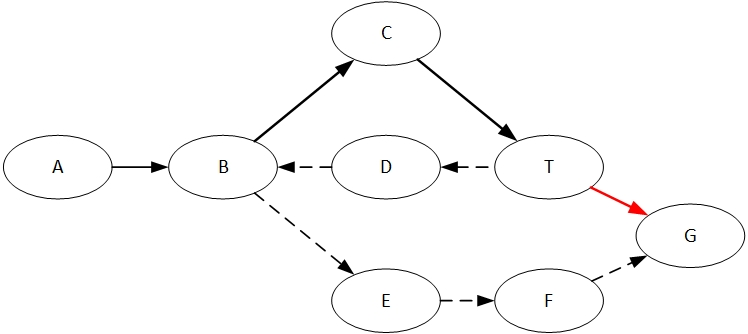
\includegraphics[width=120mm,scale=1]{figs/TransferRouting}
	\caption{Routing Transfers in Raiden Network \cite{rad:001}}
	\label{fig:TR}
\end{figure}

\vspace{0.5cm}
\subsubsection{Raiden API}	\label{R-API}	
Raiden has a URL encoded RESTFUL API that allows users to interact with Raiden nodes. Raiden accepts and returns JSON-encoded objects. The API path has this format textbf{/api/<version>/}. Each Raiden endpoint can be interacted with using one of the HTTP methods e.g GET, PUT, POST, PATCH etc. . Raiden defines three types of objects: A channel object for uniquely identifying a channel on the Raiden Network, an event object for uniquely identifying channel events, and error object for returning errors for any unsuccessful API queries \cite{rad:001}. Detailed documentation about API endpoints is given in \cite{rad:001}. Some important API queries and endpoints are briefly described below:

\textbf{Registering ERC20 Tokens:} A token can be registered by calling the textit{/tokens} end point with the contract address of the token. Registering deploys a token network contract for that token \cite{rad:001}. This API end point has the following format: 

\textbf{$PUT /api/(version)/tokens/(tokenAddress)$} \cite{rad:001}

\textbf{Channel Deployment:} A channel is deployed by calling the \textit{/channels} endpoint of Raiden rest API with the correct ERC20 token address along with the partner address with whom the channel will be established \cite{rad:001}. This API end point has the following format: 

\textbf{$PUT /api/(version)/channels$} \cite{rad:001}

\textbf{Funding:} A channel can be funded by either or both parties by transferring and locking tokens in the channel. The channel is opened by calling the \textit{/channels} with channel object as payload \cite{rad:001}. An example of opening a payment channel is given below: 
\begin{lstlisting}[language=Java,frame=single,tabsize=2,showspaces=false,showstringspaces=false,
  keywordstyle=\color{blue},morekeywords={function,returns,constant,memory},caption={Opening a Payement Channel on Raiden \cite{rad:001}}]
PUT /api/1/channels HTTP/1.1
Host: localhost:5001
Content-Type: application/json

{
    "partner_address": "0x61C808D82A3Ac53231750daDc13c777b59310bD9",
    "token_address": "0xEA674fdDe714fd979de3EdF0F56AA9716B898ec8",
    "total_deposit": 35000000,
    "settle_timeout": 500
}
\end{lstlisting}
\textbf{Payment:} Either participant can initiate a payment by calling the \textit{/payments} endpoint using the http POST request \cite{rad:001}. The API end point has the following format:

\textbf{$POST /api/(version)/payments/(tokenAddress)/(targetAddress)$} \cite{rad:001}
%\clearpage

\vspace{0.5cm}
\subsection{InterPlanetary File System (IPFS)} \label{IPFS}
\subsubsection{Motivation - Case for decentralized Repository} \label{motivation}
Supply Chain Management Processes generate large amounts of data in the form of shipping manifests, order histories, custom invoices, and shipment logs. These logs are vital for documentation, compliance and analytics purposes. They stream line existing processes and help in planning more efficient solutions for the future. These reasons make it necessary to have a complete and in-depth log of every activity in the Supply Chain Cycle. The initial iteration of the Supply Chain Dapp was using Ethereum blockchain to store everything including data, conditions, and logs. However, initial testing and evaluation of individual submodules soon revealed that storing large chunks of data on a public blockchain such as Ethereum becomes prohibitively expensive (see \ref{TrxCost}) and is hence unsuitable for most companies.
\vspace{0.5cm}
\subsubsection{IPFS}

The problems mentioned in section \ref{motivation} motivated the search for alternate solutions to serve as a decentralized repository for storing data and logs. The ideal solution needs to be decentralized so as not to introduce a single point of failure in an otherwise decentralized environment. It should provide easy read access to all participants, while preventing unauthorized writes or edits. Interplanetary File system or IPFS \cite{DBLP:journals/corr/Benet14} is a peer to peer hypermedia protocol that aims to be a decentralized replacement for most common Internet protocols like HTTP and FTP etc. These protocols determine the core architecture of most modern centralized applications on the internet. IPFS satisfies all the requirements described earlier.  It is designed as a content addressable decentralized replacement for the web. A content-addressed distributed network such as IPFS has many benefits: It decouples data from servers and replicates them across the network of nodes. Data can be stored close to the user. It allows users to verify the integrity of data in the presence of untrusted hosts and protects against DDoS attacks \cite{DBLP:journals/corr/Benet14}. IPFS can be seen as single BitTorrent swarm exchanging objects inside a git repository. It provides a high performance block storage model with content-addressed hyperlinks for building file systems, decentralized applications, blockchains and even permanent web pages \cite{DBLP:journals/corr/Benet14}. Detailed design and description for internal working of IPFS can be found in \cite{DBLP:journals/corr/Benet14}. A brief summary of important building blocks of IPFS is given below:

\textbf{Identities:} Nodes are identified by their NodeID, which is a hash of their public key. IPFS uses S/Kademlia’s static puzzle to generate a pair of public and private keys. The keys are encrypted with a passphrase and stored on the node. Nodes exchange public keys with their peers and verify each other identities by calculating the hash of the public key and checking if it matches peers NodeID \cite{DBLP:journals/corr/Benet14}.

\textbf{Network:} This module manages connections to other peers using various underlying protocols. It provides a number of desirable primitives to insure smooth functioning of the IPFS network. It uses SCTP to provide reliability, even when the underlying network is unreliable. It provides authenticity and integrity of data by using checksums and HMACs. Finally, connectivity in all network environments is insured by employing ICE NAT traversal techniques \cite{DBLP:journals/corr/Benet14}.

\textbf{Routing:} IPFS uses a DSHT based routing system to find peers that can serve particular objects. The DHT is created using S/kademlia and coral \cite{DBLP:journals/corr/Benet14}.

\textbf{Objects:} Objects in IPFS are quickly hashed and stored in a Merkle Dag data structure. This insures that objects, that contain the same content, are stored only once and that all content and their links are uniquely identifiable through content addressing scheme. IPFS uses directed acyclic graphs to store links between objects as cryptographic hashes \cite{DBLP:journals/corr/Benet14}.
   
\textbf{Files:} Files are stored in a versioned filesystem created on top of Merkle DAG. IPFS file objects are modeled on Git objects and as such are very close to them in design \cite{DBLP:journals/corr/Benet14}.

\textbf{Naming:} IPFS uses a mutable naming system called IPNS to store and address mutable objects and content. Without IPNS it would be necessary to communicate new hash address with other nodes every time content was changed in a mutable object. IPFS achieves this by defining a mutable state. Every user is assigned a mutable namespace of the form \textit{/ipns/NodeID} \cite{DBLP:journals/corr/Benet14}. Users can publish an object to this path by signing it with their private key. Other users can retrieve the object and verify its integrity by checking the signature of the uploader.  Mutable objects cannot be content-addressed, hence IPFS relies on its routing system to publish their hashes and counts on state distribution through the network for other nodes to find mutable objects \cite{DBLP:journals/corr/Benet14}.
 

